%
% tikztemplate.tex -- template for standalon tikz images
%
% (c) 2019 Prof Dr Andreas Müller, Hochschule Rapperswil
%
\documentclass[tikz]{standalone}
\usepackage{amsmath}
\usepackage{times}
\usepackage{txfonts}
\usepackage{pgfplots}
\usepackage{csvsimple}
\usetikzlibrary{arrows,intersections,math}
\begin{document}
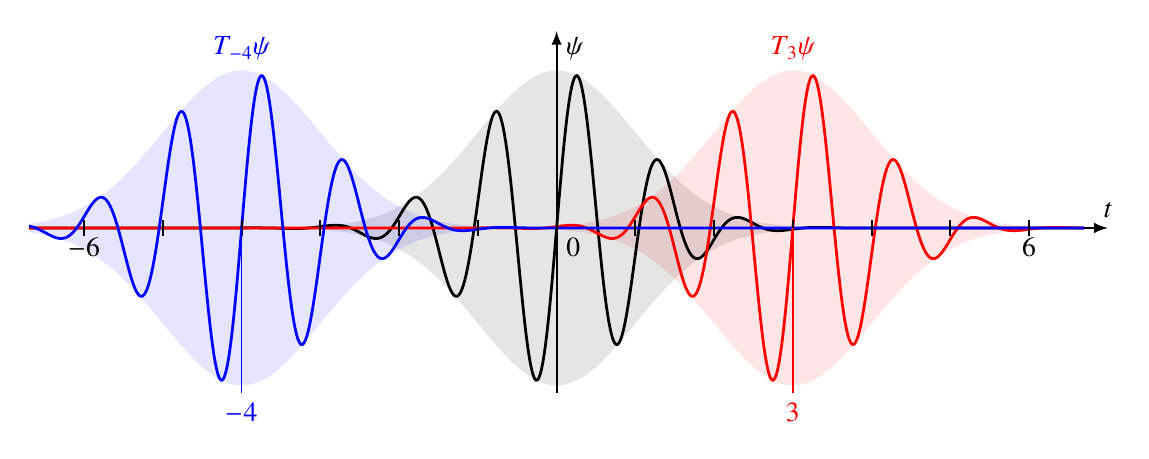
\begin{tikzpicture}[>=latex]

\def\pivalue{3.14159}
\def\frequency{6}

\fill[color=gray!20] 
	plot[domain=-4:4,samples=200]
		({\x},{2*exp(-(\x*\x/2))}) --
	plot[domain=4:-4,samples=200]
		({\x},{-2*exp(-(\x*\x/2))})
	--cycle;

\def\offsetone{3}
\fill[color=red!10] 
	plot[domain={\offsetone-4}:{\offsetone+4},samples=200]
		({\x},{2*exp(-((\x-\offsetone)*(\x-\offsetone)/2))}) --
	plot[domain={\offsetone+4}:{\offsetone-4},samples=200]
		({\x},{-2*exp(-((\x-\offsetone)*(\x-\offsetone)/2))})
	--cycle;

\node[color=red] at ({\offsetone},2) [above] {$T_{\offsetone}\psi$};
\definecolor{redgray}{rgb}{0.9,0.8,0.8}
\fill[color=redgray]
	plot[domain={\offsetone-4}:{\offsetone/2},samples=100]
		({\x},{2*exp(-((\x-\offsetone)*(\x-\offsetone)/2))}) --
	plot[domain={\offsetone/2}:4,samples=100]
		({\x},{2*exp(-(\x*\x/2))}) --
	plot[domain=4:{\offsetone/2},samples=100]
		({\x},{-2*exp(-(\x*\x/2))}) --
	plot[domain={\offsetone/2}:{\offsetone-4},samples=100]
		({\x},{-2*exp(-((\x-\offsetone)*(\x-\offsetone)/2))}) -- cycle;

\def\offsetone{-4}
\fill[color=blue!10] 
	plot[domain=-6.7:{\offsetone+4},samples=200]
		({\x},{2*exp(-((\x-\offsetone)*(\x-\offsetone)/2))}) --
	plot[domain={\offsetone+4}:-6.7,samples=200]
		({\x},{-2*exp(-((\x-\offsetone)*(\x-\offsetone)/2))})
	--cycle;
\node[color=blue] at ({\offsetone},2) [above] {$T_{\offsetone}\psi$};
\definecolor{bluegray}{rgb}{0.8,0.8,0.9}
\fill[color=bluegray]
	plot[domain=-6.7:{\offsetone/2},samples=100]
		({\x},{2*exp(-(\x*\x/2))}) --
	plot[domain={\offsetone/2}:4,samples=100]
		({\x},{2*exp(-((\x-\offsetone)*(\x-\offsetone)/2))}) --
	plot[domain=4:{\offsetone/2},samples=100]
		({\x},{-2*exp(-((\x-\offsetone)*(\x-\offsetone)/2))}) --
	plot[domain={\offsetone/2}:-6.7,samples=100]
		({\x},{-2*exp(-(\x*\x/2))}) -- cycle;


\draw[->,line width=0.7pt] (-6.7,0)--(7.0,0) coordinate[label=$t$];
\draw[->,line width=0.7pt] (0,-2.1)--(0,2.5);
\node at (0,2) [above right] {$\psi$};

\draw[line width=1pt] plot[domain=-6.7:6.7,samples=800]
	({\x},{2*sin(\frequency*\x*(180/\pivalue))*exp(-(\x*\x/2))});

\def\offsetone{3}
\draw[line width=1pt,color=red] plot[domain=-6.7:6.7,samples=800]
	({\x},{2*sin(\frequency*(\x-\offsetone)*(180/\pivalue))*exp(-((\x-\offsetone)*(\x-\offsetone)/2))});

\def\offsetone{-4}
\draw[line width=1pt,color=blue] plot[domain=-6.7:6.7,samples=800]
	({\x},{2*sin(\frequency*(\x-\offsetone)*(180/\pivalue))*exp(-((\x-\offsetone)*(\x-\offsetone)/2))});

\foreach \x in {-6,...,6}{
	\draw[line width=0.7pt] ({\x},-0.1)--({\x},0.1);
}

\node at (6,0) [below] {$6$};
\node at (0,0) [below right] {$0$};
\node at (-6,0) [below] {$-6$};

\draw[line width=0.5pt,color=blue] (-4,0)--(-4,-2.1);
\node[color=blue] at (-4,-2.1) [below] {$-4$};
\draw[line width=0.5pt,color=red] (3,0)--(3,-2.1);
\node[color=red] at (3,-2.1) [below] {$3$};

\end{tikzpicture}
\end{document}

